\chapter{New Revolutions in Particle Physics: Spontaneous Symmetry Breaking, Goldstone Bosons, and Gauge Invariance}

These notes follow Leonard Susskind's Lecture 7 in the supplementary \emph{Particle Physics 2: Standard Model} track, with curation by LazyingArt LLC. The lecture begins with a very explicit target: we want to understand how a photon-like particle can acquire mass. But Susskind does not start by writing down the Higgs mechanism. He starts more carefully. Before one can even formulate that mechanism, one has to understand two mathematical ideas: spontaneous symmetry breaking and gauge invariance. The order matters. First we learn how a symmetry can be present in the equations and absent in the ground state; then we learn what changes when the symmetry is local rather than global.

\section{The Road to a Massive Gauge Boson}

The lecture is organized around a problem. A gauge boson, like the photon, seems to resist an ordinary mass term. If we simply write down a mass by hand, gauge invariance is destroyed. So we proceed indirectly. We first return to the simpler idea of spontaneous symmetry breaking in systems with degenerate ground states. From there we move to a complex scalar field with a continuous \(U(1)\) symmetry, where the broken phase produces a massless Goldstone mode. Only after that do we ask the sharper question: can the same \(U(1)\) symmetry be made local, so that the phase may vary from point to point?

That is the logical route of the lecture. It is not a digression away from the Higgs phenomenon. It is the preparation without which the Higgs phenomenon would be only a slogan.

\section{Discrete Breaking: Magnets, Bias, and the Domain Wall}

Susskind reopens the discussion with the simplest magnetic model. Each spin can point either up or down, and neighboring spins save energy by aligning. There is no intrinsic asymmetry between the all-up state and the all-down state. The equations respect the reflection
\[
\uparrow \longleftrightarrow \downarrow.
\]
Nevertheless, once the system is cooled into its ground state, it does not remain in some neutral middle position. It chooses.

That is the first meaning of spontaneous symmetry breaking here. The symmetry is present in the underlying description, but the lowest-energy configuration settles into one of several degenerate possibilities. A tiny perturbation very far away can choose the orientation of the entire sample. The system is unstable to arbitrarily small bias because the alternatives are exactly degenerate.

Explicit symmetry breaking is different. If an external magnetic field points upward, then up and down are no longer equal from the start. The asymmetry is not produced by the ground state; it is already built into the energy function. Then a single distant spin cannot persuade a macroscopic sample to reverse itself, because flipping a large region against the external field costs energy proportional to the volume of the wrong-way region.

\subsection{Question \& Answer}

\paragraph{Question.} How can we tell spontaneous symmetry breaking from explicit symmetry breaking?

\paragraph{Answer.} The lecture answers this operationally. Take a large sample. Freeze the spins on the left boundary upward and the spins on the right boundary downward. Then compare what the lowest-energy configuration does in the bulk.

If the asymmetry is explicit, for example because there is a magnetic field throughout the sample favoring up, then the down-oriented boundary can penetrate only a finite distance. A macroscopic region of wrong-way spins would cost too much energy. There is no stable central interface.

If the symmetry is only spontaneously broken, then up and down are equally good in the bulk. In that case the lowest-energy state subject to the boundary conditions can contain two macroscopic domains, one up and one down, separated by a transition region. That interface is the domain wall. Its existence is the diagnostic of the spontaneously broken discrete symmetry.

\begin{figure}[t]
\centering
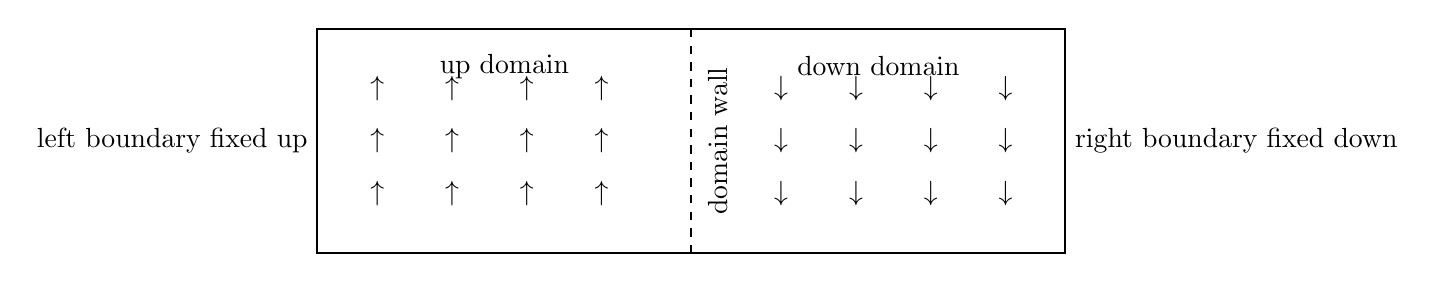
\begin{tikzpicture}[scale=0.95]
\draw[thick] (0,0) rectangle (10,3);
\draw[dashed,thick] (5,0) -- (5,3);
\node at (2.5,2.5) {up domain};
\node at (7.5,2.5) {down domain};
\node[rotate=90] at (5.35,1.5) {domain wall};
\foreach \x in {0.8,1.8,2.8,3.8}{
  \node at (\x,0.8) {$\uparrow$};
  \node at (\x,1.5) {$\uparrow$};
  \node at (\x,2.2) {$\uparrow$};
}
\foreach \x in {6.2,7.2,8.2,9.2}{
  \node at (\x,0.8) {$\downarrow$};
  \node at (\x,1.5) {$\downarrow$};
  \node at (\x,2.2) {$\downarrow$};
}
\node[left] at (0,1.5) {left boundary fixed up};
\node[right] at (10,1.5) {right boundary fixed down};
\end{tikzpicture}
\caption{Boundary conditions that reveal the discrete domain wall. In the spontaneously broken case both orientations are equally good in the bulk, so a macroscopic interface can survive.}
\label{fig:lecture07-domain-wall}
\end{figure}

\section{The Field-Theory Translation}

The lecture then translates the magnetic story into field theory. Instead of discrete spins, let us consider a real scalar field \(\phi\). In relativistic notation the simplest model is
\begin{equation}
\mathcal{L}=\frac12\,\partial_\mu\phi\,\partial^\mu\phi - V(\phi).
\label{eq:real-scalar-lagrangian}
\end{equation}
The corresponding energy density has the schematic form
\begin{equation}
\mathcal{E}=\frac12\,\dot{\phi}^{\,2}+\frac12\,(\nabla\phi)^2+V(\phi).
\label{eq:real-scalar-energy}
\end{equation}

The discrete symmetry is now
\[
\phi \longrightarrow -\phi.
\]
If \(V(\phi)\) is symmetric and has two equal minima at \(\phi=\pm f\), then there are two constant ground states:
\[
\phi(x)=+f,
\qquad
\phi(x)=-f.
\]
This is the continuum analogue of the all-up and all-down magnetic states.

The new point is that the domain wall is now understood through gradient energy. Suppose we insist on boundary conditions that place the field at \(+f\) on one side of space and at \(-f\) on the other. Why can the field not simply jump? The answer is already visible in \eqref{eq:real-scalar-energy}. A sharp jump means a large spatial derivative. In one dimension, for example, the wall energy contains
\begin{equation}
E_{\text{grad}} \sim \int dx\, \frac12\left(\frac{d\phi}{dx}\right)^2.
\label{eq:gradient-wall}
\end{equation}
A discontinuous or nearly discontinuous change makes this term very large. The field therefore spreads the transition out over a finite region. The wall is not a literal discontinuity. It is a finite interpolation region forced on us by the gradient term.

The lecture also contrasts this with an unbroken potential having a unique minimum at \(\phi=0\). In that case the symmetric point is itself the ground state. Then the vacuum does not choose between equivalent alternatives, because there are no distinct degenerate alternatives to choose from.

We can now restate the earlier distinction in field-theory language. Spontaneous breaking means a symmetric Lagrangian with several degenerate minima. Explicit breaking means that the potential is tilted so that one side is energetically preferred already at the level of the Lagrangian.

\section{The Complex Field and Global \(U(1)\)}

Up to this point the symmetry has been discrete. That is not the symmetry of most gauge theories. The Standard Model lives instead with continuous groups such as \(U(1)\), \(SU(2)\), and \(SU(3)\). So the lecture now turns to the simplest continuous example.

Let \(\phi\) be a complex field,
\begin{equation}
\phi=\phi_R+i\phi_I,
\qquad
\phi^*=\phi_R-i\phi_I,
\qquad
\phi^*\phi=\phi_R^2+\phi_I^2.
\label{eq:complex-components}
\end{equation}
This is a field whose values live in an internal plane, not in physical space. The point \((\phi_R,\phi_I)\) rotates under multiplication by a phase.

\begin{figure}[t]
\centering

\includegraphics[width=0.78\textwidth]{lecture_07_figure_02.png}
\caption{Complex field components and phase rotation on the \(\phi\)-plane. The board separates the component decomposition from the rotationally invariant combination \(\phi^*\phi\).}
\label{fig:lecture07-complex-board}
\end{figure}

The natural kinetic term is
\begin{equation}
\mathcal{L}=\partial_\mu\phi^*\,\partial^\mu\phi - V(\phi^*\phi).
\label{eq:complex-lagrangian}
\end{equation}
We choose a single consistent phase convention throughout these notes:
\begin{equation}
\phi' = e^{i\theta}\phi,
\qquad
\phi^{*\prime}=e^{-i\theta}\phi^*,
\label{eq:global-u1}
\end{equation}
with \(\theta\) constant. The lecture checks signs on the board more than once, but the invariant content is this: a constant phase rotation is a symmetry.

Indeed, because \(\theta\) is constant,
\[
\partial_\mu\phi' = e^{i\theta}\partial_\mu\phi,
\qquad
\partial_\mu\phi^{*\prime}=e^{-i\theta}\partial_\mu\phi^*,
\]
so the phase factors cancel in the product \(\partial_\mu\phi^*\partial^\mu\phi\). Likewise \(V\) remains invariant provided it depends only on \(\phi^*\phi\).

\begin{figure}[t]
\centering
\begin{tikzpicture}[scale=1.1]
\draw[->] (-2.3,0) -- (2.6,0) node[right] {$\phi_R$};
\draw[->] (0,-2.1) -- (0,2.4) node[above] {$\phi_I$};
\draw[thick,->] (0,0) -- (1.55,0.9);
\draw[thick,->] (0,0) -- (1.15,1.4);
\draw[thick] (0.7,0) arc[start angle=0,end angle=38,radius=0.7];
\node at (0.95,0.32) {$\theta$};
\node[below right] at (1.55,0.9) {$\phi$};
\node[above right] at (1.15,1.4) {$e^{i\theta}\phi$};
\end{tikzpicture}
\caption{Clean internal-space picture of the global \(U(1)\) action: multiplication by a phase rotates the field in the \((\phi_R,\phi_I)\)-plane.}
\label{fig:lecture07-complex-tikz}
\end{figure}

At this point the lecture compares two potentials.

First, the symmetric unbroken case:
\[
V(\phi^*\phi)=\phi^*\phi.
\]
Its minimum lies at \(\phi=0\), the origin of the internal plane. Since the origin is invariant under rotation, the vacuum does not break the \(U(1)\) symmetry.

Second, the broken case:
\begin{equation}
V(\phi^*\phi)=-a\,\phi^*\phi+b(\phi^*\phi)^2,
\qquad a,b>0.
\label{eq:mexican-hat}
\end{equation}
Near the origin the negative quadratic term drives the field away from zero, while the positive quartic term stabilizes the growth at large radius. The minimum is therefore not at a point but on a circle,
\begin{equation}
\phi^*\phi=f^2.
\label{eq:vacuum-circle}
\end{equation}
The potential is still rotationally symmetric, but the ground state must choose one point on the circle. This is spontaneous breaking of a continuous symmetry.

\subsection{Question \& Answer}

\paragraph{Question.} Are there domain walls for a continuously broken symmetry?

\paragraph{Answer.} Not in the same sense as in the discrete case. Fix the field to point in direction \(A\) at one end of a large sample and in direction \(B\) at the other. A sharp jump from \(A\) to \(B\) would again create a large gradient energy, so it is not preferred. But now there is a new option that did not exist for a reflection symmetry: the field can move continuously along the vacuum circle from one direction to the other. The cheapest configuration therefore stays on the trough and changes its angle gradually across space.

The lecture is careful here. If \(A\) and \(B\) are not diametrically opposite, one direction around the circle is shorter than the other, and that is the energetically preferred path. Susskind remarks that one can justify the linear interpolation of the angle by a simple calculus-of-variations argument. The essential point is simpler: the continuously broken symmetry replaces the discrete wall by a smooth low-energy mode.

\begin{figure}[t]
\centering
\begin{tikzpicture}[scale=0.95]
\begin{scope}
\draw[->] (-3.2,0) -- (3.2,0) node[right] {$x$};
\fill ( -2.7,0) circle (1.3pt);
\fill (  2.7,0) circle (1.3pt);
\node[below] at (-2.7,0) {$x_L$};
\node[below] at (2.7,0) {$x_R$};
\draw[thick] (-2.7,1.2) .. controls (-1.3,1.2) and (0.2,0.6) .. (1.5,0.1) .. controls (2.1,-0.1) and (2.45,-0.05) .. (2.7,0.1);
\node at (-1.85,1.55) {$\alpha(x)$};
\end{scope}
\begin{scope}[xshift=8.2cm]
\draw (0,0) circle (2);
\fill (1.55,1.25) circle (1.4pt) node[above right] {$A$};
\fill (-0.55,1.92) circle (1.4pt) node[above] {$B$};
\draw[line width=1.2pt] (1.55,1.25) arc[start angle=39,end angle=106,radius=2];
\node at (0.95,2.35) {vacuum track};
\end{scope}
\end{tikzpicture}
\caption{Smooth interpolation for the continuously broken symmetry. Across space the angle changes gradually; in field space the motion follows the vacuum circle from \(A\) to \(B\).}
\label{fig:lecture07-smooth-interpolation}
\end{figure}

\section{Goldstone Bosons from Motion Along the Vacuum Manifold}

The lecture now turns the smooth interpolation into a particle. The bridge is the long-wavelength criterion for masslessness. If a field configuration varies like
\begin{equation}
\varphi(x)\sim e^{ikx},
\label{eq:plane-wave}
\end{equation}
then \(k\) plays the role of momentum. A massive mode still stores energy when \(k\to 0\), because even a homogeneous displacement costs potential energy. A massless mode does not: when only gradient energy remains, the energy of a very long wavelength excitation tends to zero as \(k\to 0\).

That is exactly what the broken continuous symmetry provides. Motion along the trough changes the field without climbing the potential.

To make this explicit, rewrite the complex field in polar variables:
\begin{equation}
\phi=\rho e^{i\alpha}.
\label{eq:polar-field}
\end{equation}
Here \(\rho\) is the radial field and \(\alpha\) is the angular field. They are themselves spacetime-dependent fields. Differentiating \eqref{eq:polar-field} gives
\begin{align}
\partial_\mu\phi
&=
e^{i\alpha}\big(\partial_\mu\rho+i\rho\,\partial_\mu\alpha\big),
\label{eq:dphi-polar}
\\
\partial_\mu\phi^*
&=
e^{-i\alpha}\big(\partial_\mu\rho-i\rho\,\partial_\mu\alpha\big).
\label{eq:dphistar-polar}
\end{align}
Multiplying the two, the cross terms cancel:
\begin{equation}
\partial_\mu\phi^*\,\partial^\mu\phi
=
(\partial_\mu\rho)(\partial^\mu\rho)+\rho^2(\partial_\mu\alpha)(\partial^\mu\alpha).
\label{eq:polar-kinetic}
\end{equation}
The lecture writes the result schematically as
\begin{equation}
\mathcal{L}=(\partial\rho)^2+\rho^2(\partial\alpha)^2 - V(\rho),
\label{eq:rho-alpha-lagrangian}
\end{equation}
where \(V(\rho)\) is shorthand for a potential depending only on the radial degree of freedom. More precisely, it is inherited from \(V(\phi^*\phi)=V(\rho^2)\), but the crucial point is that \(\alpha\) does not appear in the potential.

\begin{figure}[t]
\centering

\includegraphics[width=0.88\textwidth]{lecture_07_figure_03.png}
\caption{Polar-field Lagrangian and symmetry-breaking potential as presented on the board. The boxed low-energy angular term and the Mexican-hat sketch appear together.}
\label{fig:lecture07-polar-board}
\end{figure}

Now specialize to low-energy configurations. If the field remains near the minimum of the broken potential, then \(\rho\) hardly moves away from the vacuum radius:
\[
\rho \approx f.
\]
Substituting this into \eqref{eq:rho-alpha-lagrangian} gives
\begin{equation}
\mathcal{L}_{\text{low }E}\approx f^2(\partial_\mu\alpha)(\partial^\mu\alpha).
\label{eq:goldstone-alpha}
\end{equation}
Since \(f\) is only a constant, we may absorb it into the field by defining
\begin{equation}
\beta=f\alpha.
\label{eq:beta-def}
\end{equation}
Then
\begin{equation}
\mathcal{L}_{\text{low }E}\approx (\partial_\mu\beta)(\partial^\mu\beta),
\label{eq:beta-massless}
\end{equation}
which is the Lagrangian of a massless field, up to conventional normalization factors.

This is the Goldstone mode. It is nothing mysterious: it is the angular motion along the vacuum manifold.

\begin{figure}[t]
\centering
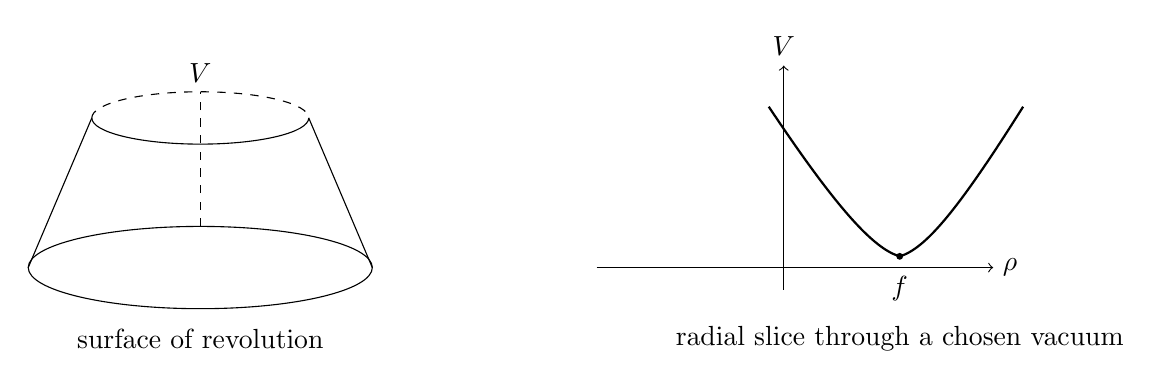
\begin{tikzpicture}[scale=0.95]
\begin{scope}
\draw (0,0) ellipse (2.3 and 0.55);
\draw (-2.3,0) -- (-1.45,2.0);
\draw (2.3,0) -- (1.45,2.0);
\draw (-1.45,2.0) arc[start angle=180,end angle=360,x radius=1.45,y radius=0.35];
\draw[dashed] (-1.45,2.0) arc[start angle=180,end angle=0,x radius=1.45,y radius=0.35];
\draw[dashed] (0,0.55) -- (0,2.35);
\node at (0,2.6) {$V$};
\node at (0,-0.95) {surface of revolution};
\end{scope}
\begin{scope}[xshift=7.8cm]
\draw[->] (-2.5,0) -- (2.8,0) node[right] {$\rho$};
\draw[->] (0,-0.3) -- (0,2.7) node[above] {$V$};
\draw[thick] (-0.2,2.15) .. controls (0.7,0.8) and (1.2,0.25) .. (1.55,0.15)
                         .. controls (1.9,0.25) and (2.35,0.8) .. (3.2,2.15);
\fill (1.55,0.15) circle (1.3pt);
\node[below] at (1.55,0.02) {$f$};
\node at (1.55,-0.95) {radial slice through a chosen vacuum};
\end{scope}
\end{tikzpicture}
\caption{Clean reconstruction of the broken potential: a circular trough of minima and a radial slice showing the restoring force in the \(\rho\) direction.}
\label{fig:lecture07-mexican-hat}
\end{figure}

Two qualitatively different modes are now visible.

First, the angular mode \(\alpha\). A homogeneous shift of \(\alpha\) just moves the field from one point on the circle to another. There is no restoring force, and the only energy comes from gradients. Its quanta are therefore massless.

Second, the radial mode \(\rho\). If we displace the field radially away from the trough, the potential pulls it back. A homogeneous radial displacement oscillates with nonzero frequency. That nonzero zero-momentum oscillation energy is what we interpret as a mass.

The lecture then broadens the point with analogies. Spin waves in a ferromagnet are Goldstone modes of broken rotational symmetry. A long elastic string, translated uniformly up and down in the absence of gravity, has a translation symmetry; long-wavelength waves on the string are Goldstone modes of that symmetry. A slinky or a uniform medium supports sound waves for essentially the same reason: an overall translation costs no energy, while a slowly varying translation from place to place costs only a little gradient energy.

\begin{figure}[t]
\centering

\includegraphics[width=0.68\textwidth]{lecture_07_figure_04.png}
\caption{Long-wavelength Goldstone-wave sketch used in the discussion of spin waves and related analogies.}
\label{fig:lecture07-wave-board}
\end{figure}

\begin{figure}[t]
\centering
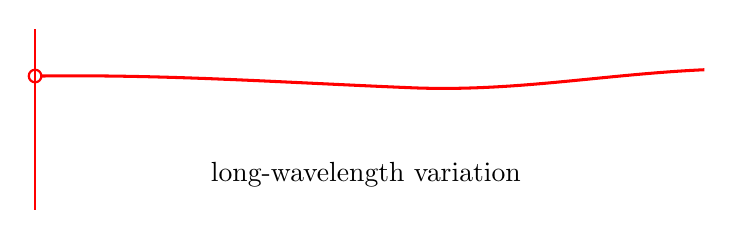
\begin{tikzpicture}[scale=1.0]
\draw[red,thick] (0,0) -- (0,2.3);
\draw[red,thick] (0,1.7) circle (0.08);
\draw[red,line width=1.1pt] (0.08,1.7)
  .. controls (1.7,1.72) and (3.1,1.62) .. (4.8,1.55)
  .. controls (6.1,1.5) and (7.2,1.72) .. (8.5,1.78);
\node at (4.2,0.45) {long-wavelength variation};
\end{tikzpicture}
\caption{A clean schematic of the slowly varying profile emphasized in the lecture: the energy becomes small when the variation is spread over a long distance.}
\label{fig:lecture07-wave-tikz}
\end{figure}

What matters in all these examples is the same structural fact. There is a symmetry transformation which costs no energy when performed uniformly, and therefore a very gradual position-dependent version of that transformation costs only a little energy. That is the pattern behind Goldstone bosons.

\section{Local \(U(1)\), the Covariant Derivative, and the Forbidden Mass Term}

At this stage the lecture pivots sharply. Up to now the phase rotation has been global: the same \(\theta\) everywhere. But the gauge-theory question is stronger. Can the phase be rotated differently at different points of spacetime?

\subsection{Question \& Answer}

\paragraph{Question.} Can a local phase rotation be made into a symmetry?

\paragraph{Answer.} Not with ordinary derivatives alone. If
\[
\phi'(x)=e^{i\theta(x)}\phi(x),
\]
then differentiating the phase produces new terms involving \(\partial_\mu\theta\), and the kinetic term changes. The lecture's answer is that we can restore the symmetry only by introducing a new field \(A_\mu\) and replacing the ordinary derivative by a covariant derivative. The new field is not optional decoration. It is the compensating field that makes the local symmetry possible.

Let us see the obstruction first. Take
\begin{equation}
\phi'(x)=e^{i\theta(x)}\phi(x).
\label{eq:local-transform}
\end{equation}
Then
\begin{align}
\partial_\mu\phi'
&=
e^{i\theta}\big(\partial_\mu\phi+i(\partial_\mu\theta)\phi\big),
\label{eq:dphi-prime}
\\
\partial_\mu\phi^{*\prime}
&=
e^{-i\theta}\big(\partial_\mu\phi^*-i(\partial_\mu\theta)\phi^*\big).
\label{eq:dphistar-prime}
\end{align}
Multiplying them, the phases cancel but unwanted derivative terms remain:
\begin{equation}
\partial_\mu\phi^{*\prime}\,\partial^\mu\phi'
=
\partial_\mu\phi^*\,\partial^\mu\phi
+i\big(\phi\,\partial_\mu\phi^*-\phi^*\,\partial_\mu\phi\big)\partial^\mu\theta
+\phi^*\phi\,\partial_\mu\theta\,\partial^\mu\theta.
\label{eq:local-failure}
\end{equation}
So the potential \(V(\phi^*\phi)\) is still invariant, but the derivative term is not. This is the disaster Susskind emphasizes on the board: local phase rotations are not symmetries of the original kinetic term.

The repair is to introduce a gauge field \(A_\mu\) and choose a consistent transformation rule
\begin{equation}
A'_\mu=A_\mu-\partial_\mu\theta.
\label{eq:A-transform}
\end{equation}
The lecture checks the signs mid-derivation; we fix this convention once and for all because it makes the cancellation transparent. We then define the covariant derivatives
\begin{equation}
D_\mu\phi=\partial_\mu\phi+iA_\mu\phi,
\qquad
D_\mu\phi^*=\partial_\mu\phi^*-iA_\mu\phi^*.
\label{eq:covariant-derivatives}
\end{equation}
Now compute the transformed covariant derivative:
\begin{align}
D_\mu\phi'
&=
\partial_\mu\phi'+iA'_\mu\phi'
\nonumber\\
&=
e^{i\theta}\big(\partial_\mu\phi+i(\partial_\mu\theta)\phi\big)
+i\big(A_\mu-\partial_\mu\theta\big)e^{i\theta}\phi
\nonumber\\
&=
e^{i\theta}\big(\partial_\mu\phi+iA_\mu\phi\big)
=
e^{i\theta}D_\mu\phi.
\label{eq:covariant-transform}
\end{align}
Similarly,
\begin{equation}
D_\mu\phi^{*\prime}=e^{-i\theta}D_\mu\phi^*.
\label{eq:covariant-transform-conj}
\end{equation}
Therefore the phase factors cancel in the product \(D_\mu\phi^*D^\mu\phi\), exactly as they did in the global theory.

\begin{figure}[t]
\centering

\includegraphics[width=0.84\textwidth]{lecture_07_figure_05.png}
\caption{Covariant derivatives and the assembled gauge-invariant gauge-field terms. The right board keeps the cleaned final formulas, while the left board preserves part of the intermediate phase-transformation work.}
\label{fig:lecture07-gauge-board}
\end{figure}

At this point the lecture assembles the gauge-invariant scalar-plus-gauge theory. The board suppresses conventional normalization factors, and the precise sign of the Maxwell term depends on the metric convention, but the standard form is
\begin{equation}
\mathcal{L}
=
D_\mu\phi^*\,D^\mu\phi
-
V(\phi^*\phi)
-
\frac14 F_{\mu\nu}F^{\mu\nu},
\label{eq:gauge-lagrangian}
\end{equation}
with
\begin{equation}
F_{\mu\nu}=\partial_\mu A_\nu-\partial_\nu A_\mu.
\label{eq:field-strength}
\end{equation}
This object is gauge invariant because
\begin{align}
F'_{\mu\nu}
&=
\partial_\mu A'_\nu-\partial_\nu A'_\mu
\nonumber\\
&=
\partial_\mu\big(A_\nu-\partial_\nu\theta\big)
-
\partial_\nu\big(A_\mu-\partial_\mu\theta\big)
\nonumber\\
&=
F_{\mu\nu}
-
\partial_\mu\partial_\nu\theta
+
\partial_\nu\partial_\mu\theta
=
F_{\mu\nu}.
\label{eq:F-invariant}
\end{align}
Its mixed time-space components give the electric field, and its space-space components give the magnetic field. This is the Maxwell piece of the theory.

What, then, is forbidden? The lecture ends by emphasizing the crucial obstruction:
\begin{equation}
\Delta\mathcal{L}_{\text{mass}}
=
\frac12 m^2 A_\mu A^\mu.
\label{eq:forbidden-mass}
\end{equation}
This would be the direct mass term for a photon-like vector field. But it is not gauge invariant, because \(A_\mu\) does not transform homogeneously:
\[
A_\mu A^\mu \neq A'_\mu A^{\mu\prime}.
\]
So a gauge boson cannot simply be given a mass by hand. The real photon is massless precisely because the \(U(1)\) gauge symmetry is exact. But the lecture refuses to end there. Susskind's final move is the cliffhanger: perhaps spontaneous symmetry breaking can do what a bare mass term cannot. In the next lecture that is exactly what will happen. The Goldstone mode will disappear from the physical spectrum, and the gauge field will acquire a mass. That is the Higgs phenomenon.

\section{Summary and the Next Step}

The lecture has now built the two ingredients it promised at the start. First, spontaneous symmetry breaking means that the equations may be symmetric even while the ground state chooses one configuration from a degenerate set. For a discrete symmetry this gives domain walls; for a continuous symmetry it gives a smooth low-energy direction in field space and therefore Goldstone bosons.

Second, gauge invariance is a stronger notion than global symmetry. A spacetime-dependent phase rotation is not a symmetry of the ordinary kinetic term, but it becomes one after we introduce the compensating field \(A_\mu\) and replace \(\partial_\mu\) by \(D_\mu\). The resulting theory is gauge invariant, but precisely because it is gauge invariant it forbids a direct mass term \(\tfrac12 m^2 A_\mu A^\mu\).

So we end exactly where the lecture intends us to end: with a paradox that is now mathematically sharp. Continuous spontaneous symmetry breaking seems to produce an unwanted massless Goldstone boson, while gauge invariance forbids a hand-made mass for the gauge field. The Higgs phenomenon will solve both problems at once, but that solution belongs to the next chapter.